%************************************************
% Beispielaufgaben
%************************************************
\chapter{Beispielaufgaben}
\label{sec:exercises}

Die Anwendungsmöglichkeiten der Software sollen im Folgenden durch eine Reihe von Beispielaufgaben verdeutlicht werden. Die Aufgaben sind nicht geeignet von Schülern alleine gelöst zu werden. Es bedarf einer ausführlichen Einführung und die in den Aufgaben benötigten Konzepte müssen vorab durch eine Lehrkraft erklärt werden. Zusätzlich zum Bildschirmfoto der Musterlösung steht ein Video zur Verfügung, indem die Musterlösung gebaut und ausgeführt wird. Die Musterlösungen stellen i.~d.~R. nur eine von vielen Wegen dar die Aufgabe zu lösen.

\section{Aufgabe 1}
\label{sec:exercises:1}

Dein Lastwagen ist bereits beladen. Fahre zum Ablageplatz und lade den Container ab. Löse die Aufgabe, indem Du zwei Befehle hintereinander ausführst.

\begin{description}[noitemsep]
  \item[Welt wählen:] Welt A
  \item[Du brauchst:] Befehle
  \item[Video:] \url{https://vimeo.com/315544834} (Passwort: trucklino)
\end{description}

\begin{figure}[H]
  \begin{subfigure}[b]{0.40\textwidth}
    \includegraphics[width=\textwidth]{gfx/exercises-world-a.png}
    \caption{Welt A}
  \end{subfigure}\hfill
  \begin{subfigure}[b]{0.40\textwidth}
    
\includegraphics[width=\textwidth]{gfx/exercises-program-1.png}
    \caption{Musterlösung zu Aufgabe 1}
  \end{subfigure}\hfill
  \caption{Welt und Musterlösung zu Aufgabe 1}
\end{figure}

\pagebreak

\section{Aufgabe 2}
\label{sec:exercises:2}

Dieses Mal musst Du die Fracht erst aufladen. Dein Weg enthält außerdem eine Kurve. Reihe mehrere Befehle aneinander, um die Aufgabe zu lösen.

\begin{description}[noitemsep]
  \item[Welt wählen:] Welt B
  \item[Du brauchst:] Befehle
  \item[Video:] \url{https://vimeo.com/315545287} (Passwort: trucklino)
\end{description}

\begin{figure}[H]
  \begin{subfigure}[b]{0.40\textwidth}
    \includegraphics[width=\textwidth]{gfx/exercises-world-b.png}
    \caption{Welt B}
  \end{subfigure}\hfill
  \begin{subfigure}[b]{0.40\textwidth}
    \includegraphics[width=\textwidth]{gfx/exercises-program-2.png}
    \caption{Musterlösung zu Aufgabe 2}
  \end{subfigure}\hfill
  \caption{Welt und Musterlösung zu Aufgabe 2}
\end{figure}

\pagebreak

\section{Aufgabe 3}
\label{sec:exercises:3}

Erkennst Du das Muster? Wenn Du Deine Befehle in einer Prozedur verpackst, bleibt Dein Programm kurz und übersichtlich.

\begin{description}[noitemsep]
  \item[Welt wählen:] Welt C
  \item[Du brauchst:] Befehle, eigene Prozeduren
  \item[Video:] \url{https://vimeo.com/315545769} (Passwort: trucklino)
\end{description}

\begin{figure}[H]
  \begin{subfigure}[b]{0.40\textwidth}
    \includegraphics[width=\textwidth]{gfx/exercises-world-c.png}
    \caption{Welt C}
  \end{subfigure}\hfill
  \begin{subfigure}[b]{0.40\textwidth}
    \includegraphics[width=\textwidth]{gfx/exercises-program-3.png}
    \caption{Musterlösung zu Aufgabe 3}
  \end{subfigure}\hfill
  \caption{Welt und Musterlösung zu Aufgabe 3}
\end{figure}

\pagebreak

\section{Aufgabe 4}
\label{sec:exercises:4}

Deine Prozedur kannst Du auch in einer Zählerschleife mehrmals hintereinander ausführen.

\begin{description}[noitemsep]
  \item[Welt wählen:] Welt C
  \item[Du brauchst:] Befehle, eigene Prozeduren, Zählerschleife
  \item[Video:] \url{https://vimeo.com/315545858} (Passwort: trucklino)
\end{description}

\begin{figure}[H]
  \begin{subfigure}[b]{0.40\textwidth}
    \includegraphics[width=\textwidth]{gfx/exercises-world-c.png}
    \caption{Welt C}
  \end{subfigure}\hfill
  \begin{subfigure}[b]{0.40\textwidth}
    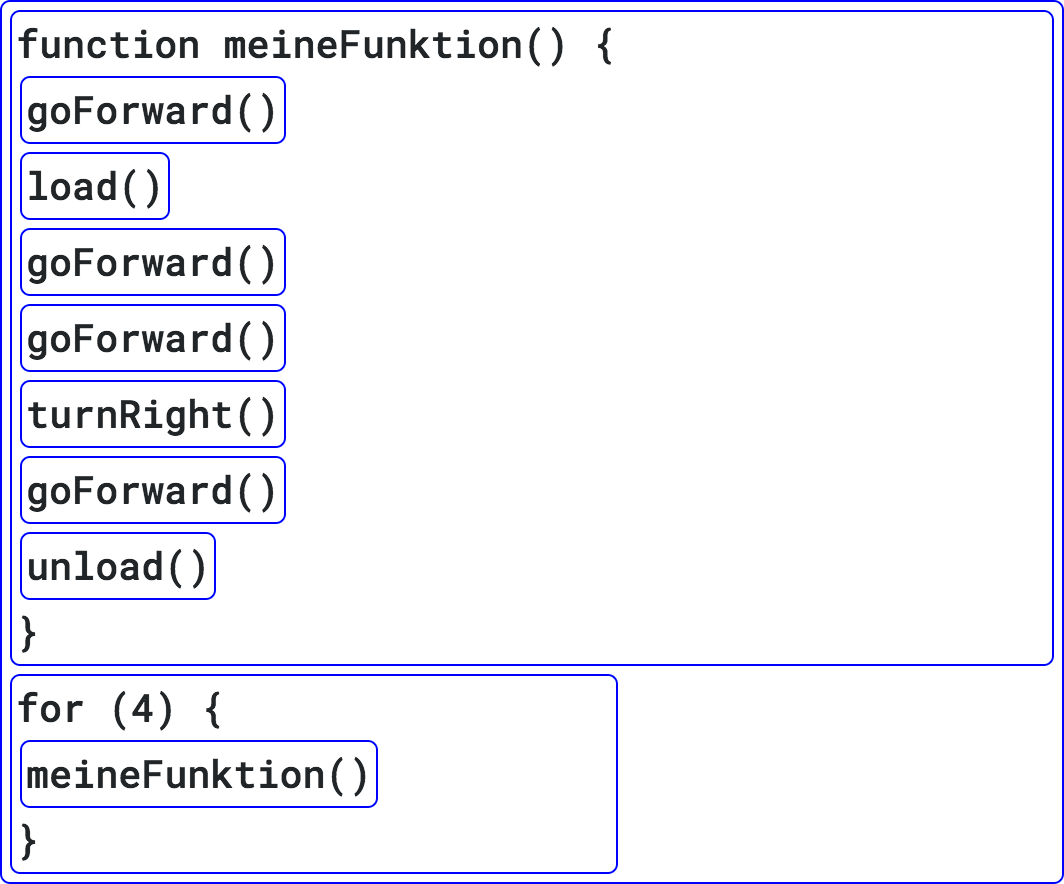
\includegraphics[width=\textwidth]{gfx/exercises-program-4.png}
    \caption{Musterlösung zu Aufgabe 4}
  \end{subfigure}\hfill
  \caption{Welt und Musterlösung zu Aufgabe 4}
\end{figure}

\pagebreak

\section{Aufgabe 5}
\label{sec:exercises:5}

Was passiert, wenn Du nicht weißt, wie oft Du Deine Prozedur ausführen musst? Benutze Sensoren und eine abweisende Schleife, um Deine Prozedur mehrmals auszuführen. Teste Dein Programm mit Welt B, C und D.

\begin{description}[noitemsep]
  \item[Welt wählen:] Welt B, Welt C, Welt D
  \item[Du brauchst:] Befehle, eigene Prozeduren, Sensoren, abweisende Schleife
  \item[Video:] \url{https://vimeo.com/315545914} (Passwort: trucklino)
\end{description}

\begin{figure}[H]
  \begin{subfigure}[b]{0.40\textwidth}
    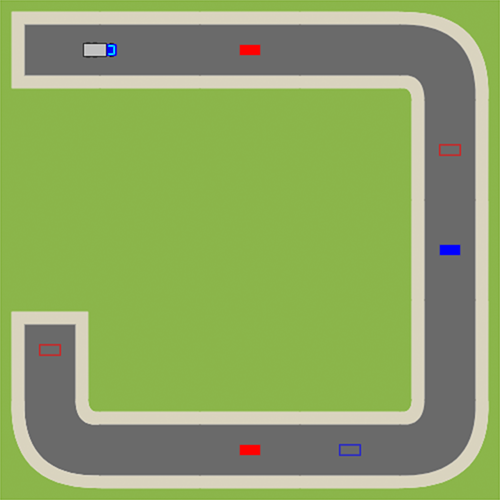
\includegraphics[width=\textwidth]{gfx/exercises-world-d.png}
    \caption{Welt D}
  \end{subfigure}\hfill
  \begin{subfigure}[b]{0.40\textwidth}
    \includegraphics[width=\textwidth]{gfx/exercises-program-5.png}
    \caption{Musterlösung zu Aufgabe 5}
  \end{subfigure}\hfill
  \caption{Welt und Musterlösung zu Aufgabe 5}
\end{figure}

\pagebreak

\section{Aufgabe 6}
\label{sec:exercises:6}

Statt einer abweisenden Schleife kannst Du auch Rekursion benutzen. Benutze eine Verzweigung, um Deine Prozedur im richtigen Moment zu verlassen.

\begin{description}[noitemsep]
  \item[Welt wählen:] Welt B, Welt C, Welt D
  \item[Du brauchst:] Befehle, eigene Prozeduren, Sensoren, Verzweigungen
  \item[Video:] \url{https://vimeo.com/315545989} (Passwort: trucklino)
\end{description}

\begin{figure}[H]
  \begin{subfigure}[b]{0.40\textwidth}
    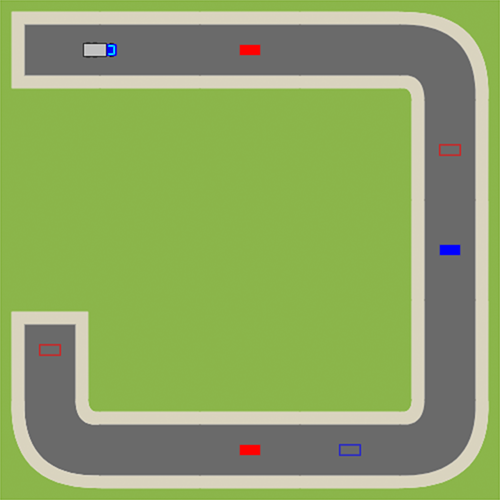
\includegraphics[width=\textwidth]{gfx/exercises-world-d.png}
    \caption{Welt D}
  \end{subfigure}\hfill
  \begin{subfigure}[b]{0.40\textwidth}
    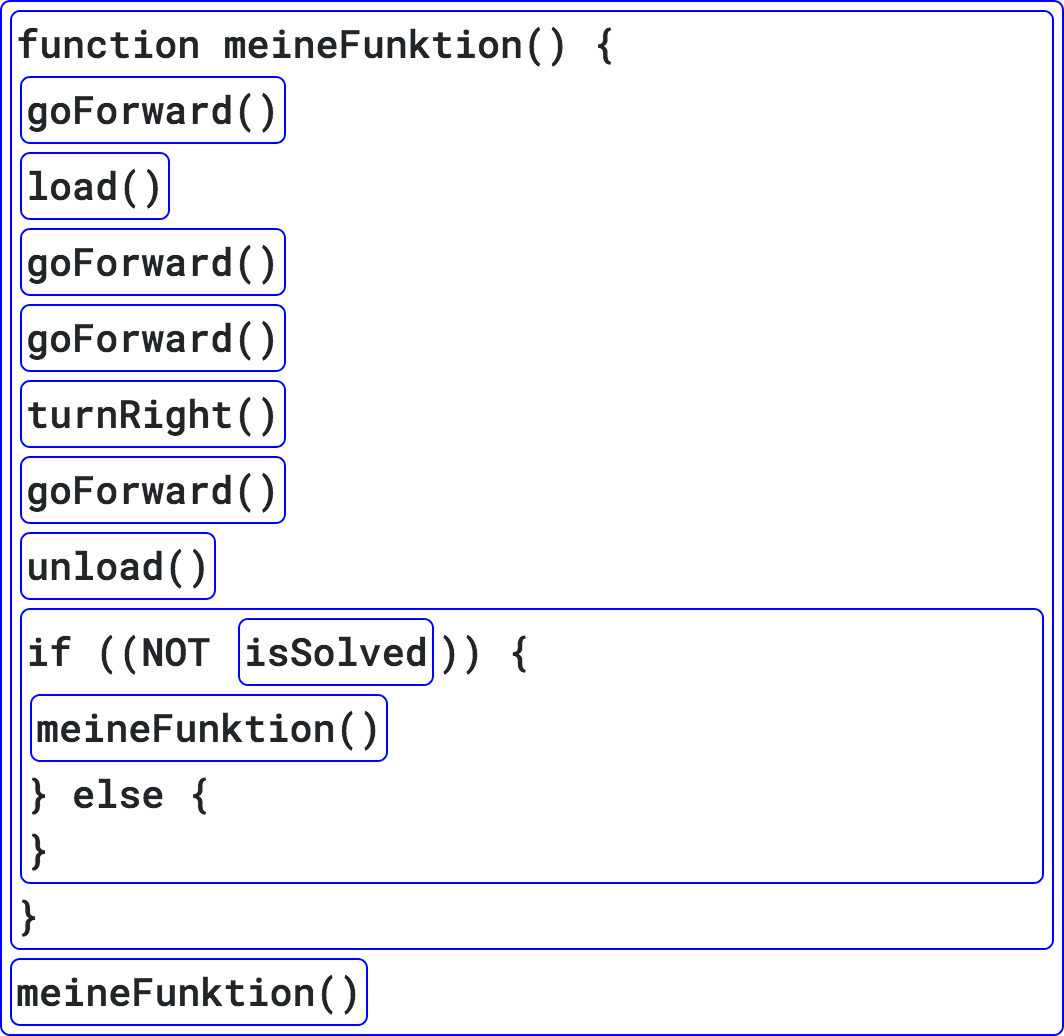
\includegraphics[width=\textwidth]{gfx/exercises-program-6.png}
    \caption{Musterlösung zu Aufgabe 6}
  \end{subfigure}\hfill
  \caption{Welt und Musterlösung zu Aufgabe 6}
\end{figure}

\pagebreak

\section{Aufgabe 7}
\label{sec:exercises:7}

Baue eine eigene Prozedur, die nicht nur geradeaus, sondern auch durch Kurven fahren kann. Deine Prozedur kannst Du solange aufrufen, bis Du am Ziel bist. Benutze dafür entweder eine abweisende Schleife oder Rekursion. Wenn Dein Programm mit Welt E funktioniert, probiere auch Welt F aus.

\begin{description}[noitemsep]
  \item[Welt wählen:] Welt E, Welt F
  \item[Du brauchst:] Befehle, eigene Prozeduren, Sensoren, Verzweigungen, abweisende Schleife (optional)
  \item[Video:] \url{https://vimeo.com/315546116} (Passwort: trucklino)
\end{description}

\begin{figure}[H]
  \begin{subfigure}[b]{0.40\textwidth}
    \includegraphics[width=\textwidth]{gfx/exercises-world-e.png}
    \caption{Welt E}
  \end{subfigure}\hfill
  \vspace{0.5cm}
  \begin{subfigure}[b]{0.40\textwidth}
    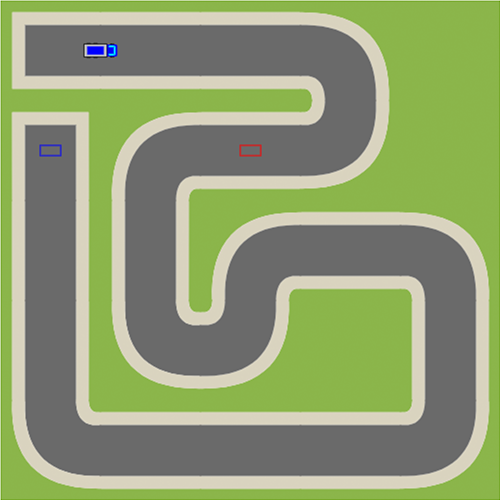
\includegraphics[width=\textwidth]{gfx/exercises-world-f.png}
    \caption{Welt F}
  \end{subfigure}
  \vspace{0.5cm}
  \begin{subfigure}[b]{0.40\textwidth}
    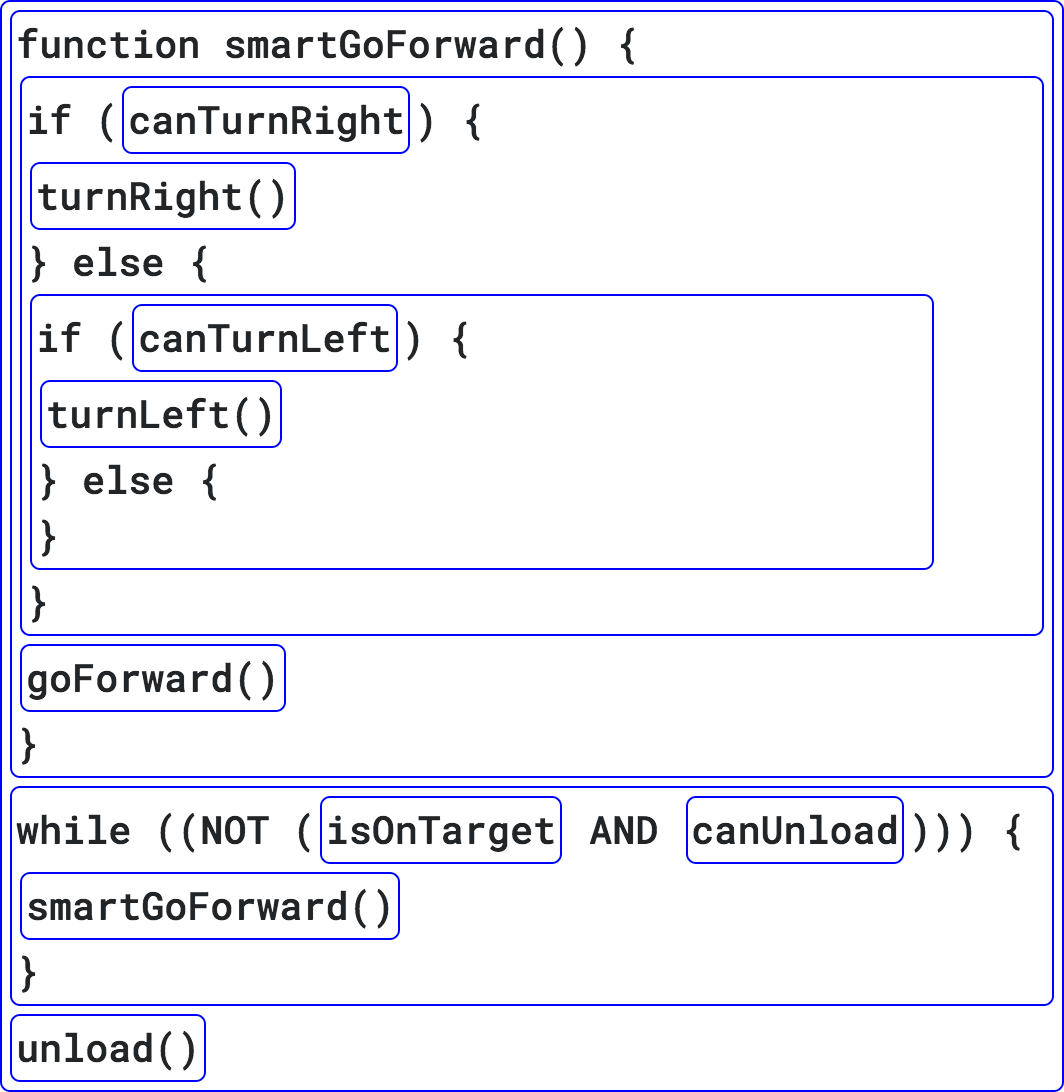
\includegraphics[width=\textwidth]{gfx/exercises-program-7.png}
    \caption{Musterlösung zu Aufgabe 7}
  \end{subfigure}
  \caption{Welten und Musterlösung zu Aufgabe 7}
\end{figure}

\pagebreak

\section{Aufgabe 8}
\label{sec:exercises:8}

Auf dem Weg sind nun einige Ampeln. Baue Dir eine zusätzliche Prozedur, die wartet, bis es grün wird.

\begin{description}[noitemsep]
  \item[Welt wählen:] Welt G
  \item[Du brauchst:] Befehle, eigene Prozeduren, Sensoren, Verzweigungen, abweisende Schleife (optional)
  \item[Video:] \url{https://vimeo.com/315546210} (Passwort: trucklino)
\end{description}

\begin{figure}[H]
  \begin{subfigure}[b]{0.40\textwidth}
    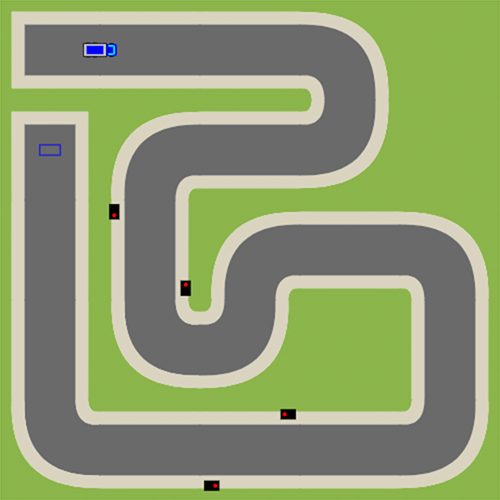
\includegraphics[width=\textwidth]{gfx/exercises-world-g.png}
    \caption{Welt G}
  \end{subfigure}\hfill
  \begin{subfigure}[b]{0.40\textwidth}
    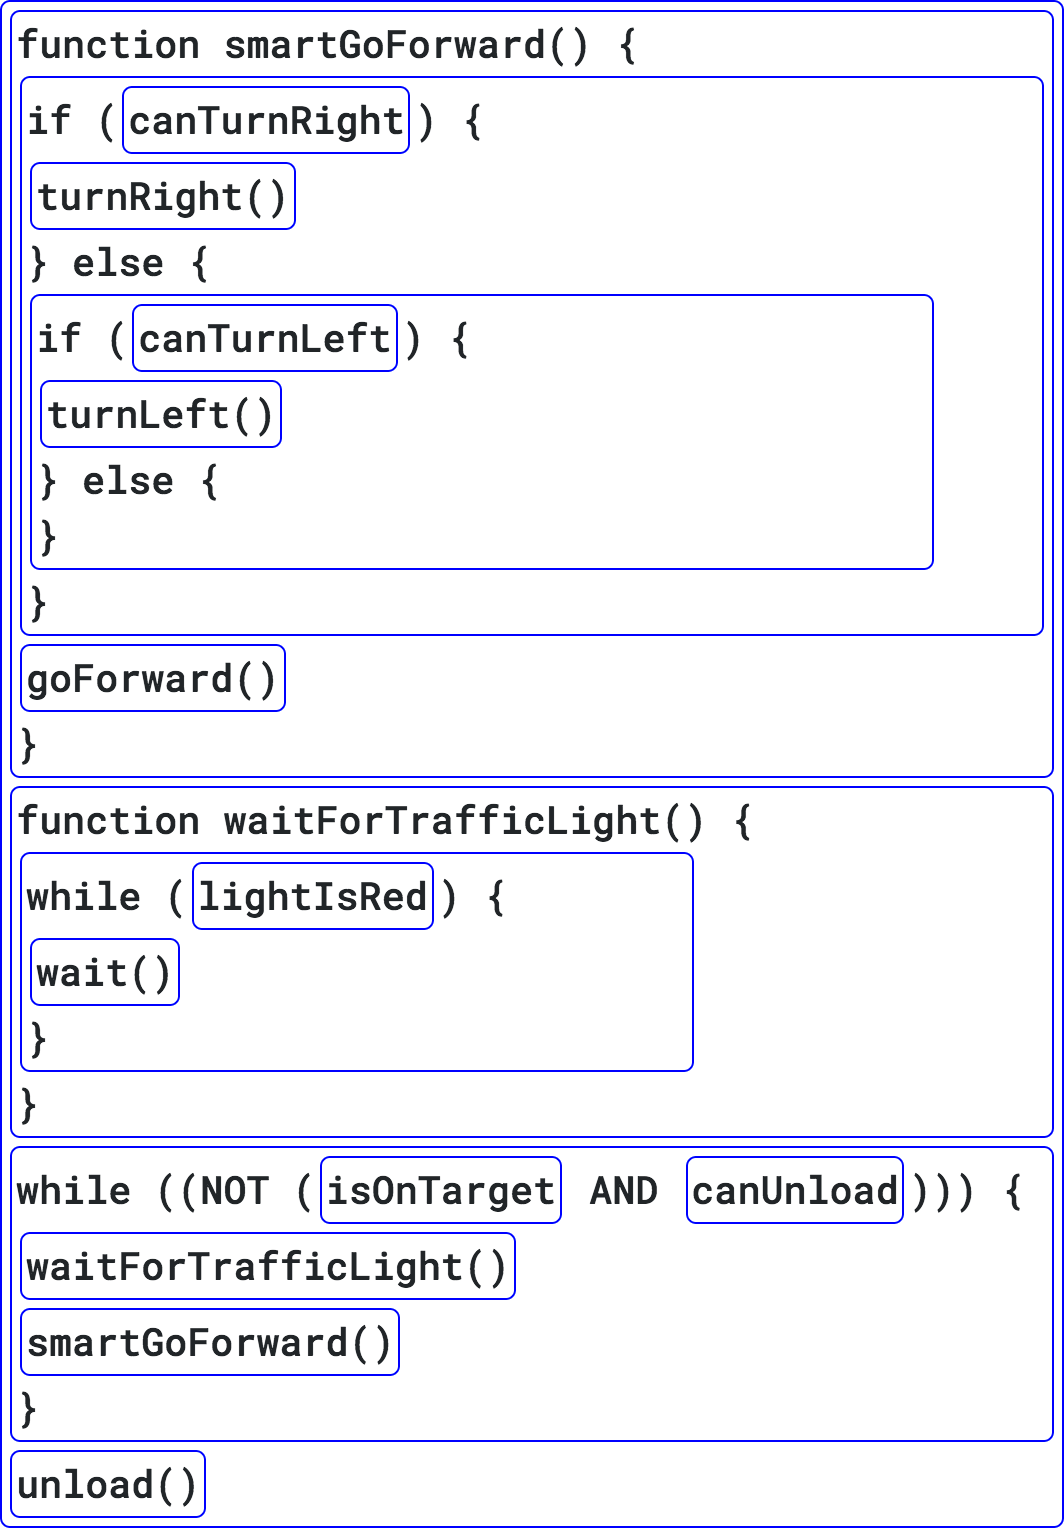
\includegraphics[width=\textwidth]{gfx/exercises-program-8.png}
    \caption{Musterlösung zu Aufgabe 8}
  \end{subfigure}\hfill
  \caption{Welt und Musterlösung zu Aufgabe 8}
\end{figure}
